\hypertarget{TreeGrow_8h}{
\section{TreeGrow.h File Reference}
\label{TreeGrow_8h}\index{TreeGrow.h@{TreeGrow.h}}
}


This graph shows which files directly or indirectly include this file:\nopagebreak
\begin{figure}[H]
\begin{center}
\leavevmode
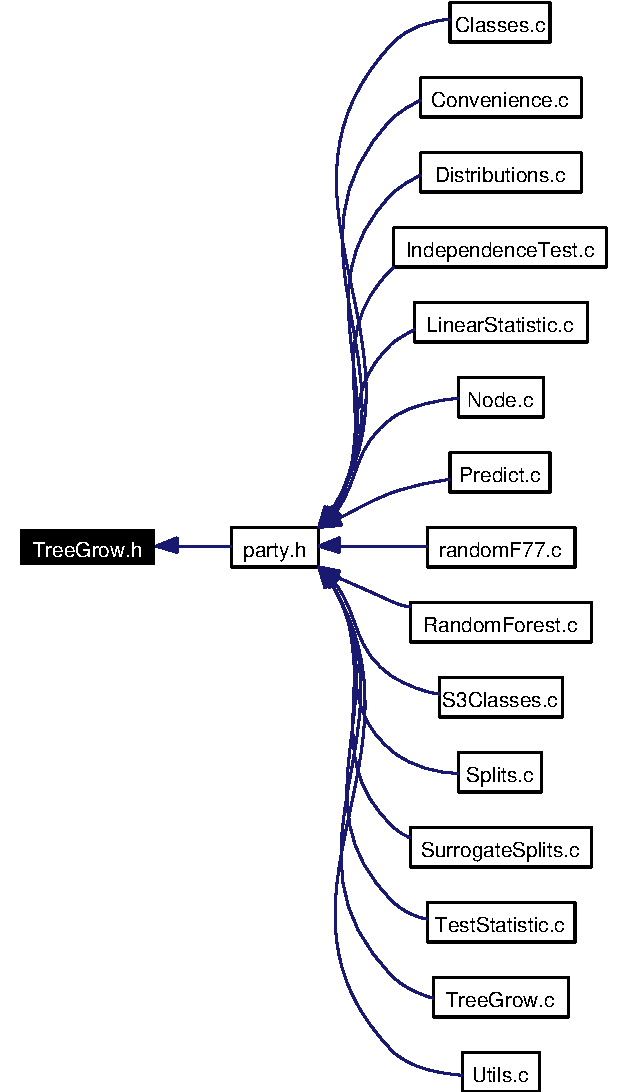
\includegraphics[width=420pt]{TreeGrow_8h__dep__incl}
\end{center}
\end{figure}
\subsection*{Functions}
\begin{CompactItemize}
\item 
void \hyperlink{TreeGrow_8h_67d352c38f59d30c7b9954bf5d3a57ad}{C\_\-TreeGrow} (SEXP node, SEXP learnsample, SEXP fitmem, SEXP controls, int $\ast$where, int $\ast$nodenum, int depth)
\end{CompactItemize}


\subsection{Function Documentation}
\hypertarget{TreeGrow_8h_67d352c38f59d30c7b9954bf5d3a57ad}{
\index{TreeGrow.h@{TreeGrow.h}!C_TreeGrow@{C\_\-TreeGrow}}
\index{C_TreeGrow@{C\_\-TreeGrow}!TreeGrow.h@{TreeGrow.h}}
\subsubsection{\setlength{\rightskip}{0pt plus 5cm}void C\_\-TreeGrow (SEXP {\em node}, SEXP {\em learnsample}, SEXP {\em fitmem}, SEXP {\em controls}, int $\ast$ {\em where}, int $\ast$ {\em nodenum}, int {\em depth})}}
\label{TreeGrow_8h_67d352c38f59d30c7b9954bf5d3a57ad}


The main tree growing function, handles the recursion. \par
 \begin{Desc}
\item[Parameters:]
\begin{description}
\item[{\em node}]a list representing the current node \item[{\em learnsample}]an object of class `LearningSample' \item[{\em fitmem}]an object of class `TreeFitMemory' \item[{\em controls}]an object of class `TreeControl' \item[{\em where}]a pointer to an integer vector of n-elements \item[{\em nodenum}]a pointer to a integer vector of length 1 \item[{\em depth}]an integer giving the depth of the current node \end{description}
\end{Desc}


Definition at line 23 of file TreeGrow.c.

References C\_\-Node(), C\_\-splitnode(), C\_\-splitsurrogate(), C\_\-surrogates(), C\_\-TreeGrow(), check\_\-depth(), get\_\-maxsurrogate(), get\_\-nobs(), get\_\-splitctrl(), get\_\-stump(), get\_\-tgctrl(), S3get\_\-leftnode(), S3get\_\-nodeterminal(), S3get\_\-nodeweights(), S3get\_\-rightnode(), and S3set\_\-nodeID().

Here is the call graph for this function:\nopagebreak
\begin{figure}[H]
\begin{center}
\leavevmode
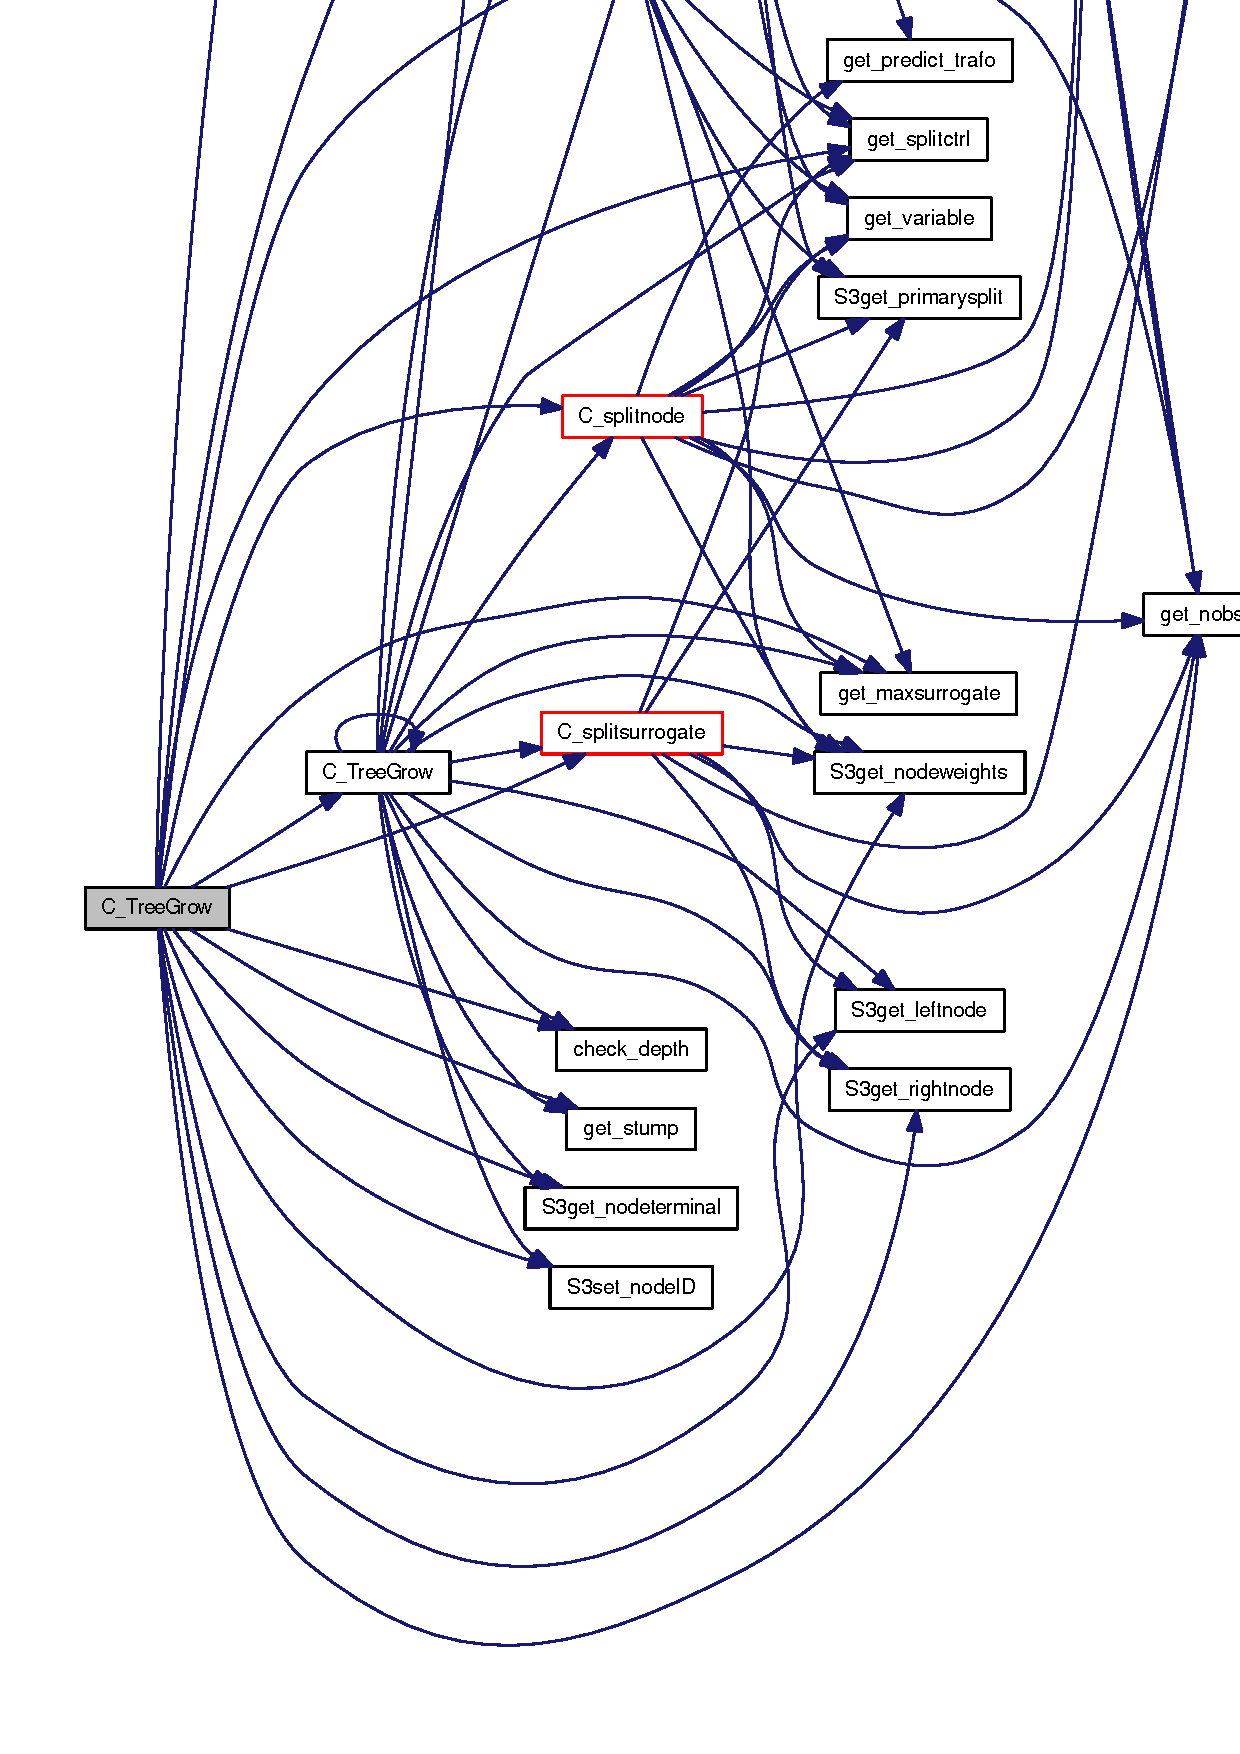
\includegraphics[width=135pt]{TreeGrow_8h_67d352c38f59d30c7b9954bf5d3a57ad_cgraph}
\end{center}
\end{figure}
